% Created 2018-05-14 Mon 05:30
% Intended LaTeX compiler: pdflatex
\documentclass[10pt]{beamer}
\usepackage[utf8]{inputenc}
\usepackage[T1]{fontenc}
\usepackage{graphicx}
\usepackage{grffile}
\usepackage{longtable}
\usepackage{wrapfig}
\usepackage{rotating}
\usepackage[normalem]{ulem}
\usepackage{amsmath}
\usepackage{textcomp}
\usepackage{amssymb}
\usepackage{capt-of}
\usepackage{hyperref}
\usetheme{Boadilla}
\author{ECON 420: Game Theory}
\date{Spring 2018}
\title{Uncertainty}
\usecolortheme{seagull}
\usefonttheme[onlylarge]{structurebold}
\usefonttheme[onlymath]{serif}
\setbeamerfont*{frametitle}{size=\normalsize,series=\bfseries}
\setbeamertemplate{navigation symbols}{}
\setbeamertemplate{itemize item}[triangle]
\setbeamertemplate{footline}{}
\setbeamertemplate{enumerate items}[default]
\hypersetup{
 pdfauthor={ECON 420: Game Theory},
 pdftitle={Uncertainty},
 pdfkeywords={},
 pdfsubject={},
 pdfcreator={Emacs 25.2.2 (Org mode 9.1.6)}, 
 pdflang={English}}
\begin{document}

\maketitle

\begin{frame}[label={sec:org282533e}]{}
\alert{Announcements} 
\begin{itemize}
\item Homework 3 on Canvas 
\begin{itemize}
\item Due \emph{Monday, May 21}
\end{itemize}
\item Reading: Chapter 8
\end{itemize}
\end{frame}

\begin{frame}[label={sec:org6f426f7}]{}
\alert{Uncertainty}
\begin{itemize}
\item So far: Strategic uncertainty
\begin{itemize}
\item Some players unaware of the actions of other players
\item Example: Simultaneous-move games
\end{itemize}
\item Today: External uncertainty
\begin{itemize}
\item "Nature" changes aspects of the game
\item Players cannot control external uncertainty, must take it into account when making decisions
\end{itemize}
\end{itemize}
\end{frame}

\begin{frame}[label={sec:org79d087b}]{}
\alert{Expected Utility Theory}
\begin{itemize}
\item Events that happen according to some probability distribution are called \emph{gambles}
\item Agents are able to rank gambles by comparing the \emph{expected utility} that they would receive from the potential outcomes of the gamble
\item The utility that we will use is \emph{von Neumann-Morgenstern (VNM)} utility
\end{itemize}
\end{frame}

\begin{frame}[label={sec:orgdb5dc03}]{}
\alert{Risk preference} 
\begin{itemize}
\item When there is uncertainty we can calculate the \emph{expected value} of a gamble
\item But people do not just consider expected value when making decisions
\item Some people might be willing to pay to avoid risk (risk aversion)
\end{itemize}
\end{frame}

\begin{frame}[label={sec:org3ec13ab}]{}
\alert{Example}
\begin{itemize}
\item Suppose I flip a coin. If heads, you get \$100. If tails, you get \$0. 
\begin{itemize}
\item What is the expected value?
\item How much would you pay to play this game?
\end{itemize}
\item Suppose instead the payoffs are \$1 million for heads, \$0 for tails.
\end{itemize}
\end{frame}

\begin{frame}[label={sec:org9743b8d}]{}
\alert{VNM Utility and Risk Preference}
\begin{itemize}
\item Outcomes are denoted \(D\) (dollars)
\item Agents in the model have preferences over outcomes represented by utility \(u=u(D)\)
\item The risk preference of the agent depends on the concavity of the utility function \(u\)
\item Agents with \emph{diminishing marginal utility} are risk averse
\begin{itemize}
\item Concave utility function
\end{itemize}
\end{itemize}
\end{frame}

\begin{frame}[label={sec:orgceb4f1d}]{Risk aversion}
\end{frame}

\begin{frame}[label={sec:org8e72400}]{Risk seeking}
\end{frame}

\begin{frame}[label={sec:orgfe61d1a}]{}
\alert{Example}
\begin{itemize}
\item A farmer's crop yield depends on weather
\item Farmer gets good weather with 50\%
\item Yield with good weather is \$160,000, yield in bad weather is \$40,000
\item Farmer has VNM utility \(u(D) = \sqrt{D}\)
\end{itemize}
\end{frame}

\begin{frame}[label={sec:org6790e51}]{}
\alert{Risk sharing}
\begin{itemize}
\item Risk averse agents willing to pay to remove risk
\item Agents can therefore benefit from trading \emph{state-contingent claims} with one another 
\begin{itemize}
\item You agree to pay someone else if you have a good outcome, someone else pays you if you have a bad outcome
\end{itemize}
\end{itemize}
\end{frame}

\begin{frame}[label={sec:org2611476}]{}
\alert{Example}
\begin{itemize}
\item Suppose there is another farmer that has the same weather probability and outcomes (weather probability is independent of first farmer)
\item Farmers agree to a contract: If one farmer gets good luck and the other gets bad luck, lucky farmer pays \$60,000 to the unlucky farmer
\item Are the farmers better off?
\end{itemize}
\end{frame}

\begin{frame}[label={sec:orgaace258}]{}
\alert{Example}
\begin{itemize}
\item Now suppose the other farmer faces no uncertainty and will earn \$100,000 with probability 1
\item The farmer with risk is willing to accept their certainty equivalence instead of the gamble
\item Is the riskless farmer willing to buy the risk in exchange for the certainty equivalence?
\end{itemize}
\end{frame}

\begin{frame}[label={sec:org7b4eed0}]{}
\alert{Example}
\begin{itemize}
\item Now suppose the farmer without risk is \emph{risk neutral}
\item What is the maximum that this farmer is willing to pay for the gamble?
\end{itemize}
\end{frame}

\begin{frame}[label={sec:org5d92c5a}]{}
\alert{Insurance and risk}
\begin{itemize}
\item Suppose there are thousands of farmers with identical risk/outcomes
\item A single entity (insurance company) can buy the risk of all of the farmers and make them better off
\item Law of large numbers says that the insurance company will earn the expected value of the gamble
\end{itemize}
\end{frame}

\begin{frame}[label={sec:org55ba178}]{}
\alert{Manipulating Risk}
\begin{itemize}
\item Sometimes agents have control over risk and can use it to their advantage
\item By increasing risk, the probability of "tail events" increases
\item This is why underdogs in sports often choose risky actions
\end{itemize}
\end{frame}

\begin{frame}[label={sec:org99e9ed5}]{}
\alert{Example}
\begin{itemize}
\item A basketball team scores 60 points per game on average
\item They are playing a better opponent and must score at least 80 points to win
\item How can this team maximize their chances of winning?
\end{itemize}
\end{frame}

\begin{frame}[label={sec:orged3689b}]{}
\alert{Cheap Talk}
\begin{itemize}
\item In coordination games, players may be able to costlessly communicate before the game begins
\item This might allow players to better coordinate on preferred outcomes
\end{itemize}
\end{frame}

\begin{frame}[label={sec:org83a93f4}]{}
\begin{center}
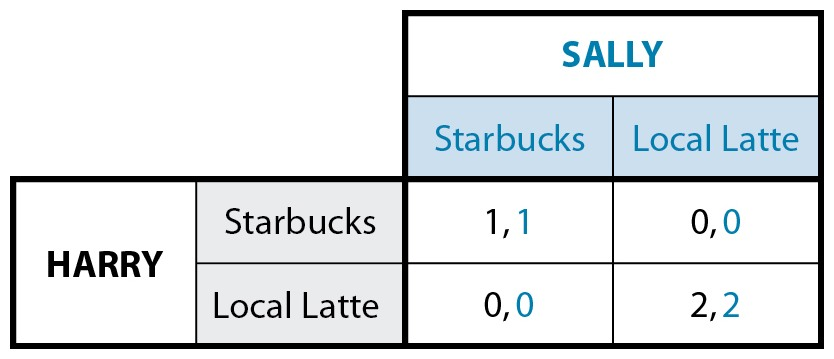
\includegraphics[width=.75\textwidth]{./img/GAMES4_FIG08.03.jpg}
\end{center}
\end{frame}
\end{document}